\section{Custom Elements}\label{custom-elements}

\begin{itemize}
\item
  TODO:
\item
  Ausformulieren:
\item
  Complete
\end{itemize}

\subsection{Einführung}\label{einfuxfchrung}

\begin{itemize}
\tightlist
\item
  Momentan: Suppe von Divs, die nicht aussagekräftig sind, siehe
  folgender Ausschnitt der Inbox der Google-Mail Webseite
  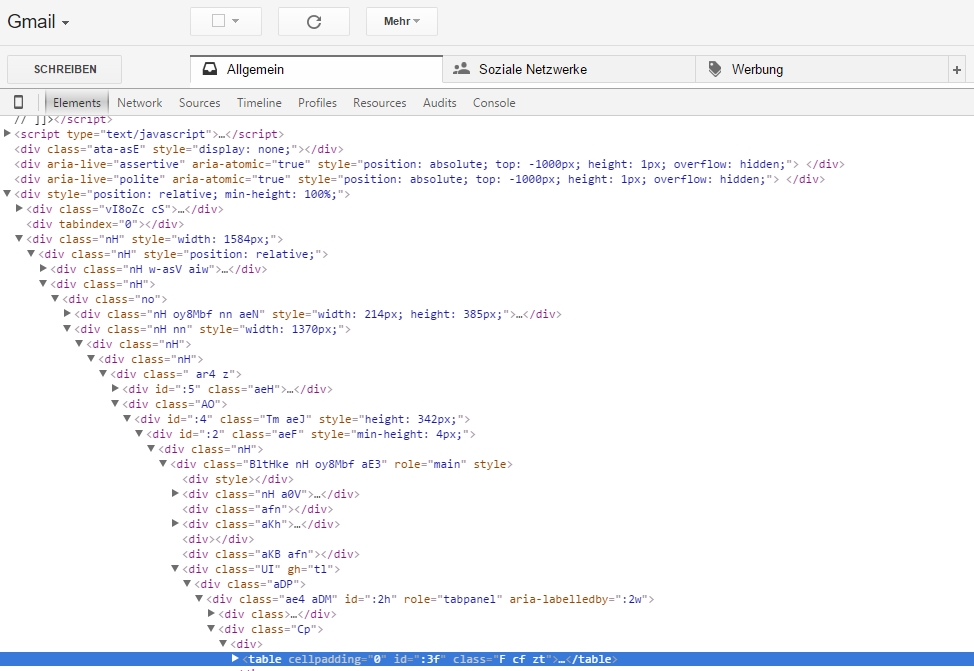
\includegraphics{images/1-custom-elements-div-suppe.jpg}
\item
  Besser: Elemente, die semantisch aussagekräftig sind. So könnte die
  Google-Mail Webseite folgender Maßen aussehen
\end{itemize}

\begin{Shaded}
\begin{Highlighting}[]
\KeywordTok{<hangout-module>}
  \KeywordTok{<hangout-chat}\OtherTok{ from=}\StringTok{"Paul, Addy"}\KeywordTok{>}
    \KeywordTok{<hangout-discussion>}
      \KeywordTok{<hangout-message}\OtherTok{ from=}\StringTok{"Paul"}\OtherTok{ profile=}\StringTok{"profile.png"}
\OtherTok{          profile=}\StringTok{"118075919496626375791"}\OtherTok{ datetime=}\StringTok{"2013-07-17T12:02"}\KeywordTok{>}
        \KeywordTok{<p>}\NormalTok{Feelin' this Web Components thing.}\KeywordTok{</p>}
        \KeywordTok{<p>}\NormalTok{Heard of it?}\KeywordTok{</p>}
      \KeywordTok{</hangout-message>}
    \KeywordTok{</hangout-discussion>}
  \KeywordTok{</hangout-chat>}
  \KeywordTok{<hangout-chat>}\NormalTok{...}\KeywordTok{</hangout-chat>}
\KeywordTok{</hangout-module>}
\end{Highlighting}
\end{Shaded}

\begin{itemize}
\tightlist
\item
  Custom Elements ermöglichen es
\item
  neue DOM Elemente zu definieren
\item
  Elemente zu definieren, die vorhandene Elemente erweitern
\item
  eigene Funktionalitäten in einem Element zu bündeln
\item
  die APIs vorhandener DOM Elemente zu erweitern
\end{itemize}

{[}Eric Bidelman 2013{]}

\subsection{Neue Elemente
registrieren}\label{neue-elemente-registrieren}

\begin{itemize}
\item
  Laut W3C Spezifikation muss ein Custom Element ein Bindestrich im
  Namen haben, z.B. \texttt{my-element}
  (http://w3c.github.io/webcomponents/spec/custom/\#concepts)
\item
  Ein neues Element wir mit der Funktion
  \texttt{var\ MyElement\ =\ document.registerElement(\textquotesingle{}my-element\textquotesingle{});}
  registriert
\item
  Als zweiter Parameter kann der \texttt{prototype} mit angegeben werden

\begin{Shaded}
\begin{Highlighting}[]
\KeywordTok{var} \NormalTok{MyElement }\OperatorTok{=} \VariableTok{document}\NormalTok{.}\AttributeTok{registerElement}\NormalTok{(}\StringTok{'my-element'}\OperatorTok{,} \OperatorTok{\{}
  \DataTypeTok{prototype}\OperatorTok{:} \VariableTok{Object}\NormalTok{.}\AttributeTok{create}\NormalTok{(}\VariableTok{HTMLElement}\NormalTok{.}\AttributeTok{prototype}\NormalTok{)}
\OperatorTok{\}}\NormalTok{)}\OperatorTok{;}
\end{Highlighting}
\end{Shaded}
\item
  Dadurch steht es in der Registry des Browsers, welche dazu verwendet
  wird um die Definitionen der Elemente aufzulösen
\item
  Nachdem das Element registriert wurde, kann es per JavaScript oder
  HTML Deklaration verwendet werden
\end{itemize}

JavaScript

\begin{Shaded}
\begin{Highlighting}[]
\KeywordTok{var} \NormalTok{myelement }\OperatorTok{=} \VariableTok{document}\NormalTok{.}\AttributeTok{createElement}\NormalTok{(}\StringTok{'my-element'}\NormalTok{)}\OperatorTok{;}
\VariableTok{document}\NormalTok{.}\VariableTok{body}\NormalTok{.}\AttributeTok{appendChild}\NormalTok{(myelement)}\OperatorTok{;}
\end{Highlighting}
\end{Shaded}

HTML

\begin{Shaded}
\begin{Highlighting}[]
\KeywordTok{<div}\OtherTok{ class=}\StringTok{"wrapper"}\KeywordTok{>}
  \KeywordTok{<my-element><my-element>}
\KeywordTok{</div>}
\end{Highlighting}
\end{Shaded}

{[}Developing Web Components 2015{]}

\subsection{Vorteile von Custom
Elements}\label{vorteile-von-custom-elements}

\begin{itemize}
\tightlist
\item
  Unangemeldete, unregistrierte Custom Tags wie z.B.
  \texttt{\textless{}myelement\textgreater{}} benutzen das Interface
  HTMLUknownElement
\item
  Angemeldete, registrierte Custom Elements wie z.B.
  \texttt{\textless{}my-element\textgreater{}} benutzen das Interface
  HTMLElement
\item
  Somit können für neue HTML Elemente eigene APIs erzeugt werden, indem
  eigene Eigenschaften und Methoden hinzugefügt werden
\end{itemize}

{[}Eric Bidelman 2015{]}

\subsubsection{Nachteil}\label{nachteil}

\begin{itemize}
\tightlist
\item
  Eventueller FOUC (Flash of unstyled content), da das Element schon im
  DOM steht, aber erst noch registriert werden muss
\item
  Kann verhindert werden, in dem man den \texttt{:unresolved}-Selector
  benutzt und die Elemente ausblendet
\end{itemize}

\texttt{my-element:unresolved\ \{\ \ \ \ \ display:\ none;\ \ \ \}}

{[}Peter Gasston 2014{]}

\subsection{Vorhandene Elemente erweitern (Type
extensions)}\label{vorhandene-elemente-erweitern-type-extensions}

\begin{itemize}
\tightlist
\item
  Statt neue Elemente zu erzeugen, können vorhandene auch erweitert
  werden
\item
  So können native HTML Elemente erweitert werden
\item
  Um einen erweitertes \texttt{button} zu erzeugen muss also folgendes
  gemacht werden:
\end{itemize}

\begin{Shaded}
\begin{Highlighting}[]
\KeywordTok{var} \NormalTok{ButtonExtendedProto }\OperatorTok{=} \VariableTok{document}\NormalTok{.}\AttributeTok{registerElement}\NormalTok{(}\StringTok{'button-extended'}\OperatorTok{,} \OperatorTok{\{}
  \DataTypeTok{prototype}\OperatorTok{:} \VariableTok{Object}\NormalTok{.}\AttributeTok{create}\NormalTok{(}\VariableTok{HTMLButtonElement}\NormalTok{.}\AttributeTok{prototype}\NormalTok{)}\OperatorTok{,}
  \DataTypeTok{extends}\OperatorTok{:} \StringTok{'button'}
\OperatorTok{\}}\NormalTok{)}\OperatorTok{;}
\end{Highlighting}
\end{Shaded}

\begin{itemize}
\tightlist
\item
  Ein erweitertes Element kann nun wie folgt vie JavaScript oder HTML
  Deklaration verwendet werden:
\end{itemize}

JavaScript:

\begin{Shaded}
\begin{Highlighting}[]
\KeywordTok{var} \NormalTok{buttonExtended  }\OperatorTok{=} \VariableTok{document}\NormalTok{.}\AttributeTok{createElement}\NormalTok{(}\StringTok{'button'}\OperatorTok{,} \StringTok{'button-extended'}\NormalTok{)}\OperatorTok{;}

\CommentTok{// Oder}

\KeywordTok{var} \NormalTok{buttonExtended }\OperatorTok{=} \KeywordTok{new} \AttributeTok{ButtonExtendedProto}\NormalTok{()}\OperatorTok{;}
\end{Highlighting}
\end{Shaded}

HTML:

\begin{Shaded}
\begin{Highlighting}[]
  \KeywordTok{<div}\OtherTok{ class=}\StringTok{"wrapper"}\KeywordTok{>}
    \KeywordTok{<button}\OtherTok{ is=}\StringTok{"button-extended"}\KeywordTok{></button>}
  \KeywordTok{</div>}
\end{Highlighting}
\end{Shaded}

{[}Eiji Kitamura 2014{]}

\subsubsection{Verwendung bei Github}\label{verwendung-bei-github}

\begin{itemize}
\tightlist
\item
  Die ``Latest commit'' Angaben eines Repositories auf Github sind ein
  erweitertes time-Element (Type Extension Custom Element mit
  time-Element)
\item
  Statt des Commit-Datums und der Zeit, wird - wenn JavaScript aktiviert
  ist - die berechnete Zeit seit dem letzten Commit angezeigt
\end{itemize}

\begin{figure}[htbp]
\centering
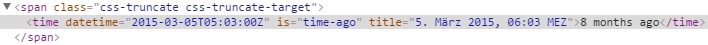
\includegraphics{images/1-custom-elements-github-time-element.jpg}
\caption{Bild: Github Einsatz eines Custom Element}
\end{figure}

\begin{itemize}
\tightlist
\item
  Dabei dient das \texttt{time} Element als Basis
\item
  Das \texttt{datetime} Attribut gibt die absolute Zeit des Commits an
\item
  \texttt{is="time-ago"} ist die Erweiterung des \texttt{time} Elements
\item
  Der Inhalt des \texttt{time} Elements zeigt die relative Zeit an
\item
  Falls der Browser nun keine Custom Elements (mit Polyfill) unterstützt
  oder JavaScript deaktiviert ist, wird dennoch das ``normale''
  \texttt{time} Element mit der absoluten Zeit angezeigt
\end{itemize}

{[}Eiji Kitamura 2014{]}

\subsection{Eigenschaften und Methoden
definieren}\label{eigenschaften-und-methoden-definieren}

\begin{itemize}
\tightlist
\item
  Custom Elements machen erst so richtig Sinn, wenn man für diese auch
  eigene Eigenschaften und Methoden definieren kann
\item
  Wie bei nativen HTML Elementen ist dies bei Custom Elements möglich,
  dies geschieht auf die gleiche Weise
\end{itemize}

\begin{Shaded}
\begin{Highlighting}[]
\CommentTok{// Methode definieren}
\VariableTok{ButtonExtendedProto}\NormalTok{.}\VariableTok{prototype}\NormalTok{.}\AttributeTok{alert} \OperatorTok{=} \KeywordTok{function} \NormalTok{() }\OperatorTok{\{}
  \AttributeTok{alert}\NormalTok{(}\StringTok{'foo'}\NormalTok{)}\OperatorTok{;}
\OperatorTok{\};}

\CommentTok{// Eigenschaft definieren}
\VariableTok{ButtonExtendedProto}\NormalTok{.}\VariableTok{prototype}\NormalTok{.}\AttributeTok{answer} \OperatorTok{=} \DecValTok{42}\OperatorTok{;}
\end{Highlighting}
\end{Shaded}

{[}Developing Web Components 2015{]}

\subsection{Custom Element Life Cycle Callbacks -
TODO?}\label{custom-element-life-cycle-callbacks---todo}

\begin{itemize}
\tightlist
\item
  Custom Elements bieten eine standardisierte API um verschiedene
  Methoden zu unterschiedlichen Zeitpunkten im ``Leben'' eines Custom
  Elements auszuführen. Diese ermöglicht es zu bestimmen, wie und wann
  ein bestimmter Code des Custom Elements ausgeführt wird.
\end{itemize}

\paragraph{createdCallback}\label{createdcallback}

\begin{itemize}
\tightlist
\item
  Wird ausgeführt, wenn eine Instanz des Custom Elements erzeugt wird.
  Beispiel:
  \texttt{document.createElement(\textquotesingle{}custom-element\textquotesingle{});}
\end{itemize}

\paragraph{attachedCallback}\label{attachedcallback}

\begin{itemize}
\tightlist
\item
  Wird ausgeführt, wenn ein Custom Element dem DOM angehängt wird.
  Beispiel: \texttt{document.body.appendChild();}
\end{itemize}

\paragraph{detachedCallback}\label{detachedcallback}

\begin{itemize}
\tightlist
\item
  Wird ausgeführt, wenn ein Custom Element aus dem DOM entfernt wird.
  Beispiel: \texttt{document.body.removeChild();}
\end{itemize}

\paragraph{attributeChangedCallback}\label{attributechangedcallback}

\begin{itemize}
\tightlist
\item
  Wird ausgeführt, wenn ein Attribut eines Custom ELements geändert
  wird. Beispiel: \texttt{MyElement.setAttribute();}
\end{itemize}

\subsubsection{\texorpdfstring{Beispiel mit
\texttt{button-extended}}{Beispiel mit button-extended}}\label{beispiel-mit-button-extended}

Anhand des \texttt{button-extended} Beispiels würde dies folgender Maßen
funktionieren:

\begin{Shaded}
\begin{Highlighting}[]
\KeywordTok{var} \NormalTok{ButtonExtendedProto }\OperatorTok{=} \VariableTok{Object}\NormalTok{.}\AttributeTok{create}\NormalTok{(}\VariableTok{HTMLElement}\NormalTok{.}\AttributeTok{prototype}\NormalTok{)}\OperatorTok{;}

\VariableTok{ButtonExtendedProto}\NormalTok{.}\AttributeTok{createdCallback} \OperatorTok{=} \KeywordTok{function}\NormalTok{() }\OperatorTok{\{}\NormalTok{...}\OperatorTok{\};}
\VariableTok{ButtonExtendedProto}\NormalTok{.}\AttributeTok{attachedCallback} \OperatorTok{=} \KeywordTok{function}\NormalTok{() }\OperatorTok{\{}\NormalTok{...}\OperatorTok{\};}

\KeywordTok{var} \NormalTok{ButtonExtended }\OperatorTok{=} \VariableTok{document}\NormalTok{.}\AttributeTok{registerElement}\NormalTok{(}\StringTok{'button-extended'}\OperatorTok{,} \OperatorTok{\{}\DataTypeTok{prototype}\OperatorTok{:} \NormalTok{ButtonExtendedProto}\OperatorTok{\}}\NormalTok{)}\OperatorTok{;}
\end{Highlighting}
\end{Shaded}

{[}Raoul Schaffranek 2014{]}

\subsection{Styling von Custom
Elements}\label{styling-von-custom-elements}

\begin{itemize}
\tightlist
\item
  Custom Elements können wie native HTML Elemente gestyled werden
\end{itemize}

\begin{Shaded}
\begin{Highlighting}[]
\NormalTok{my-element }\KeywordTok{\{}
  \KeywordTok{foo:} \NormalTok{bar}\KeywordTok{;}
\KeywordTok{\}}
\end{Highlighting}
\end{Shaded}

\begin{itemize}
\tightlist
\item
  Element-Erweiterungen können per Attribut-Selektor angesprochen werden
\end{itemize}

\begin{Shaded}
\begin{Highlighting}[]
\CharTok{[is=}\StringTok{"button-extended"}\CharTok{]} \KeywordTok{\{}
  \KeywordTok{foo:} \NormalTok{bar}\KeywordTok{;}
\KeywordTok{\}}
\end{Highlighting}
\end{Shaded}

{[}Developing Web Components 2015{]}

\subsection{Browserunterstützung}\label{browserunterstuxfctzung}

\begin{itemize}
\tightlist
\item
  Noch nicht standardtisiert, sind noch ein Working Draft
  (http://w3c.github.io/webcomponents/spec/custom/)
\item
  Deshalb bisher auch nur in Chrome und Opera unterstützt
\end{itemize}

\begin{figure}[htbp]
\centering
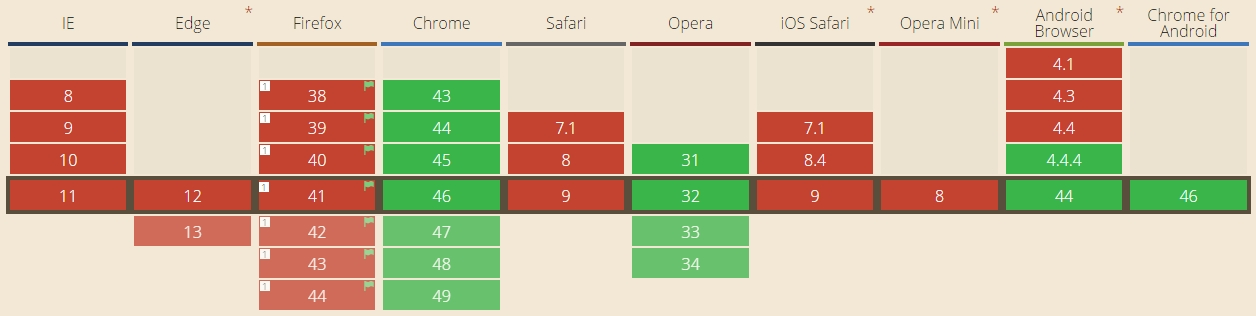
\includegraphics{images/1-custom-elements-browserunterstuetzung.jpg}
\caption{Bild: Browserunterstützung von Custom Elements}
\end{figure}

{[}Can I Use 2015{]}

\subsection{Quellen}\label{quellen}

\begin{itemize}
\tightlist
\item
  {[}Developing Web Components 2015{]} Jarrod Overson \& Jason Strimpel,
  Developing Web Components, O'Reilly 2015, S.127-138
\item
  {[}Eiji Kitamura 2014{]} Eiji Kitamura, Introduction to Custom
  Elements,
  http://webcomponents.org/articles/introduction-to-custom-elements/
\item
  http://w3c.github.io/webcomponents/spec/custom/
\item
  {[}Eric Bidelman 2013{]} Eric Bidelman, Custom Elements,
  http://www.html5rocks.com/en/tutorials/webcomponents/customelements/
\item
  {[}Can I Use 2015{]} Can I Use,
  http://caniuse.com/\#feat=custom-elements
\item
  {[}Peter Gasstton 2015{]} Peter Gasstton, A Detailed Introduction To
  Custom Elements,
  http://www.smashingmagazine.com/2014/03/introduction-to-custom-elements/
\item
  {[}Raoul Schaffranek 2014{]} Raoul Schaffranek, Web Components -- eine
  Einführung,
  https://blog.selfhtml.org/2014/12/09/web-components-eine-einfuehrung/
\end{itemize}
